\documentclass[10pt]{article}
\usepackage[margin=1in]{geometry}
\usepackage{breqn}
\usepackage{../local}


\newcommand{\classcode}{Physics 5C}
\newcommand{\classname}{Introductory Thermodynamics and Quantum Mechanics}
\renewcommand{\maketitle}{%
\hrule height4pt
\large{Eric Du \hfill \classcode}
\newline
\large{HW 10} \large{\hfill \classname \hfill} \large{\today}
\hrule height4pt \vskip .7em
\normalsize
}
\linespread{1.1}


\begin{document}
    \maketitle

    \section*{Collaborators}

        I worked with \names to complete this homework assignment.

    \section*{Problem 1}

    \begin{enumerate}[(a)]
        \item Derive expressions for the reflection and transmission coeffieints for a particle beam of energy $E$ incident on a potential down-step of height $V_0$ ($E > V_0$). Show that these coefficients are the same as those for the corrresponding case of a particle incident on an up-step, treated in Section 9-2.

        \begin{center}
            \begin{tikzpicture}
                \draw[very thick] (0,0) node[anchor=east] {$V_0$}-- (2,0) node[midway,below,yshift=-1.9cm] {I} -- (2,-2) node[anchor=north] {$0$} -- (6,-2) node[midway,below] {II} (0,1) -- (6,1) node[anchor=west] {$E$};
            \end{tikzpicture}
        \end{center}
            
        \begin{solution}
            For a down step, we can split this into two regions. Based on regions, we can write down two sets of wavefunctions: 

            \begin{align*}
                \psi_1(x) &= Ae^{ik_1x} + Be^{-ik_1x}, &&k_1 = \frac{\sqrt{2m(E - V_0)}}{\hbar}\\
                \psi_2(x) &= Ce^{ik_2x}, &&k_2 = \frac{\sqrt{2mE}}{\hbar}
            \end{align*}

            Now, we require continuity, at $x = 0$. Doing so, we obtain the following system of equations: 

            \begin{align*}
                A + B &= C \\
                ik_1(A - B) &= ik_2C
            \end{align*}

            Solving this system of equations gives us that 

            \[ C = \frac{2k_1A}{k_1 + k_2}\]

            We can calculate transmission as: 

            \begin{align*}
                T = \left| \frac{C}{A}\right|^2 \cdot \frac{V_2}{V_1} &= \left|\frac CA\right|^2 \cdot \frac{\frac{\hbar k_2}{m}}{\frac{\hbar k_1}{m}}\\
                &= \left| \frac CA\right|^2 \cdot \frac{k_2}{k_1}\\
                &= \frac{\left( \frac{2k_1A}{k_1 + k_2}\right)^2}{A^2} \cdot \frac{k_2}{k_1}\\
                &= \frac{4k_1k_2}{(k_1 + k_2)^2}
            \end{align*}

            This equation matches exactly what we expect. Furthermore, since the transmission probability is the same, then the reflection coefficient must also be the same since $R = 1-T$. 
        \end{solution}
        \item In classical particle physics there would be no reflection at a down-step (Marbles roll downstairs without hindrance.) In classical particle physics would there be a reflection at an up-step of height $V_0 < E$? What are the classical \textit{wave} analogs particle reflection at a potential down-step and a potential up-step?
        
        \begin{solution}
            If we imagine the particle as a physical ball, then for $E > V_0$ we wouldn't expect any reflection. However, if we consider the particle as a water wave splashing into a barrier, it is still possible that some of the water sloshes and makes it over the bank, an example of transmission when $E < V_0$. For a classical down-step, a classical interpretation does not exist - when a wave travels off a cliff, the water does not reflect back upstream.
        \end{solution}
    \end{enumerate}

    \pagebreak

    \section*{Problem 2}

    \begin{enumerate}[(a)]
        \item Calculate the probability current $J(x, t)$ at $x = L/2$ for the square-well sloshing state given in Eq. 8-5.
        
        \begin{solution}
            The probability current is written as: 

            \[ J(x, t) = -\frac{i\hbar}{2m}\left( \psi^\star \frac{\partial\psi}{\partial x} - \psi \frac{\partial \psi^\star}{\partial x}\right)\] 

            We know that the wavefunction is given by the equation: 

            \[ \psi(x, t) = \frac{1}{\sqrt{2}}\sqrt{\frac{2}{L}} \sin\left( \frac{\pi x}{L}\right) e^{-i\omega_1t} + \frac{1}{\sqrt{2}}\sqrt{\frac{2}{L}} \sin \left( \frac{2\pi x}{L}\right)e^{-i\omega_2t}\] 

            And so therefore, we have the terms: 

            \begin{multline*}
                \psi^\star \frac{\partial \psi}{\partial x} = \frac{\pi}{L^2} \sin \left( \frac{\pi x}{L}\right) \cos \left( \frac{\pi x}{L}\right)+ \frac{2\pi}{L^2} \sin \left( \frac{\pi x}{L}\right) \cos\left( \frac{2\pi x}{L}\right)e^{i (\omega_1 - \omega_2)t} +\\ \frac{\pi }{L^2} \sin \left( \frac{2\pi x}{L}\right) \cos \left( \frac{\pi x}{L}\right) e^{i(\omega_2 - \omega_1)t} + \frac{2\pi}{L^2} \sin \left( \frac{2\pi x}{L}\right) \cos\left( \frac{2\pi x}{L}\right)
            \end{multline*}

            Similarly, we have:

            \begin{multline*}
                \psi \frac{\partial \psi^\star}{\partial x} = \frac{\pi}{L^2} \sin \left( \frac{\pi x}{L}\right) \cos \left( \frac{\pi x}{L}\right)+ \frac{2\pi}{L^2} \sin \left( \frac{\pi x}{L}\right) \cos\left( \frac{2\pi x}{L}\right)e^{i (\omega_2 - \omega_1)t} +\\ \frac{\pi }{L^2} \sin \left( \frac{2\pi x}{L}\right) \cos \left( \frac{\pi x}{L}\right) e^{i(\omega_1 - \omega_2)t} + \frac{2\pi}{L^2} \sin \left( \frac{2\pi x}{L}\right) \cos\left( \frac{2\pi x}{L}\right)
            \end{multline*} 

            With the condition that $x = L/2$, we get that: 

            \begin{align*}
                \sin \left( \frac{\pi x}{L}\right) &= 1\\
                \cos \left( \frac{\pi x}{L}\right) &= 0\\
                \sin \left( \frac{2\pi x}{L}\right) &= 0\\
                \cos \left( \frac{2\pi x}{L}\right) &= -1
            \end{align*}

            And so therefore, we eventually get: 

            \begin{align*}
                J(L/2, t) &= -\frac{i\hbar}{2m} \left[ -\frac{2\pi}{L^2} e^{i(\omega_1 - \omega_2)t} + \frac{2\pi}{L^2} e^{i(\omega_2 - \omega_1)t}\right]\\
                &= -\frac{i\hbar}{2m} \cdot \frac{2\pi}{L^2}\left[ e^{i(\omega_2 - \omega_1)t} + e^{-i(\omega_2 - \omega_1)t}\right]\\
                &= \frac{2\pi \hbar}{mL^2} \sin((\omega_2 - \omega_1)t)
            \end{align*}
        \end{solution}
        \item This state of a particle in the square well was considered in Exercise 8-1. Verify directly that the rate at which probability disappears from the left half of the well (Exercise 8-1d) is equal to $J(x = L/2, t)$
        
        \begin{solution}
            The probability distribution for this wavefunction is given by $|\psi|^2$. From the book, we know that if $f_1$ and $f_2$ are our basis states, then we have:

            \[ \rho \equiv |\psi(x, t)|^2 = f_1^2 + f_2^2 + 2 f_1f_2 \cos\left( \frac{E_2 - E_1}{\hbar} t\right)\] 

            And so using this formula and the fact that $f_1 = \frac{1}{\sqrt{L}} \sin\left( \frac{n\pi x}{L}\right)$ and $f_2 = \frac{1}{\sqrt L} \sin\left( \frac{2\pi x}{L}\right)$, we get the equation: 

            \[ \rho = \frac{1}{L} \sin^2\left( \frac{\pi x}{L}\right) + \frac{1}{L} \sin^2 \left( \frac{2\pi x}{L}\right) + \frac{2}{L}\sin \left( \frac{ \pi x}{L}\right) \sin \left( \frac{2\pi x}{L}\right) \cos\left( \frac{E_2 - E_1}{\hbar}t\right)\] 

            Now to calculate the robability current, we need $\frac{\partial \rho}{\partial t}$, then integrate that from 0 to $L/2$. Here, we take the time derivative first because it makes our expression easier to deal with, but in principle the order does not matter. Therefore, 

            \[ \frac{\partial\rho}{\partial t} = -\frac{2}{L}\sin \left( \frac{\pi x}{L}\right) \sin \left( \frac{2 \pi x}{L}\right) \cdot \frac{E_2 - E_1}{\hbar} \left( -\sin \left( \frac{E_2 - E_1}{\hbar} t\right) \right)\] 

            The first thing we'll do is to use $E = \hbar \omega$ so we get that:

            \[ \frac{E_2 - E_1}{\hbar} = \omega_2 - \omega_1\] 

            Now taking the integral, we get: 

            \begin{align*}
                J &= -\frac{2}{L}(\omega_2 - \omega_1) \sin ((\omega_2 - \omega_1)t) \int_0^{L/2} \sin \left(\frac{\pi x}{L}\right) \sin \left( \frac{2\pi x}{L}\right) dx\\
                &= \frac{4}{3\pi} (\omega_1 - \omega_2) \sin((\omega_2 - \omega_1)t)
            \end{align*}

            Now, since this is an infinite square well, then we know that 

            \[ E_n = \frac{(n \pi \hbar)^2}{2mL^2} \implies \omega_n = \frac{n^2\pi^2 \hbar}{2mL^2}\] 

            Therefore, we can write this as: 

            \begin{align*}
                J &= \frac{4}{3\pi}\left[ \frac{\pi^2\hbar}{2mL^2} - \frac{4\pi^2}{2mL^2}\right] \sin ((\omega_2 - \omega_1)t)\\
                &= \frac{\pi\hbar}{2mL^2}\sin((\omega_2 - \omega_1)t)
            \end{align*}

            And so the expressions are the same.


        \end{solution}
    \end{enumerate}

    \pagebreak 

    \section*{Problem 3}

    Equation 9-12 relates the incident and transmitted \textit{amplitudes} for particles scattered by a one-dimensional rectangular well. 

    \begin{enumerate}[(a)]
        \item Deduce that the general expression for the transmission coefficient $T$ can be written
        
        \[ T = \frac{4k_1^2k_2^2}{4k_1^2k_2^2 + (k_2^2 - k_1^2)^2 \sin^2 k_2L}\]

        \begin{solution}
            From the book, we know that the relationship between $D$ and $A_0$ can be written as: 

            \[ 4k_1k_2 A_0 = \left[ (k_2 + k_1)^2 e^{-ik_2L} - (k_2 - k_1)^2e^{ik_2L}\right] De^{ik_1L}\] 

            Thus, this gives us the equation: 

            \[ \frac{D}{A_0} = \frac{4k_1k_2}{\left[(k_2 + k_1)^2 e^{-ik_2L} - (k_2 - k_1)^2e^{ik_2L}\right]De^{ik_1L}}\] 

            To simplify this, first we notice that when we take norm squared, that $|e^{ik_1L}|^2 = 1$, so we will omit it in our calcuoation. Let's focus on the rest of the denominator, and start simplifying it by rewriting the exponentials in terms of sines and cosines: 


            \begin{dmath*}
                (k_2 + k_1)^2 e^{-ik_2L} - (k_2 - k_1)^2 e^{ik_2L} = (k_2 + k_1)^2(\cos(k_2L) - i\sin (k_2L)) - (k_2 - k_1)^2(\cos(k_2L) + i\sin(k_2L))
            \end{dmath*}

            Then, we can group in terms of $\cos(k_2L)$ and $\sin(k_2L)$, which ultimately gives us the equation after simplification: 

            \[ \cos(k_2L)(4k_1k_2) - 2i\sin(k_2L)(k_1^2 + k_2^2)\]

            Therefore, our transmission coefficient can now be written as: 

            \begin{align*}
                \left|\frac{D}{A_0}\right|^2 &= \left| \frac{2k_1k_2}{\cos^2(k_2L)(2k_1k_2) - i\sin(k_2L)(k_1^2 + k_2^2)}\right|^2\\
                &= \frac{4k_1^2k_2^2}{\cos^2(k_2L)(4k_1^2k_2^2) + \sin^2(k_2L)(k_1^2 + k_2^2)^2}\\
                &= \frac{4k_1^2k_2^2}{(4k_1^2k_2^2)\left[\cos^2(k_2L) + \sin^2(k_2L)\right]+ \sin^2(k_2L)(k_1^2 - k_2^2)^2}\\
                &= \frac{4k_1^2k_2^2}{4k_1^2k_2^2 + (k_2^2 - k_1^2)^2 \sin^2 k_2L}
            \end{align*}

            as desired.
        \end{solution}

        \item Substituting $k_1^2 = 2mE/\hbar^2$, $k_2^2 = 2m(E + V_0)/\hbar^2$, and putting $E/V_0 = \epsilon$, show that the above expression leads to the result
        
        \[ T(\epsilon) = \frac{4\epsilon(1 + \epsilon)}{4\epsilon(1 + \epsilon) + \sin^2(\beta \sqrt{1 + \epsilon})}\] 

        where $\beta = L \sqrt{2mV_0}/\hbar$ is a dimensionless parameter characterizing the scattering well. In this form the equation for $T$ is suited for direct computations of the transmission coefficient as a function of particle energy.

        \begin{solution}
            Substituting this in, we get: 

            \begin{align*}
                T &= \frac{4 \left( \frac{2mE}{\hbar^2}\right)\left( \frac{2m(V_0 + E)}{\hbar^2}\right)}{4 \left( \frac{2mE}{\hbar^2}\right)\left( \frac{2m(V_0 + E)}{\hbar^2}\right) + \left( \frac{2mV_0}{\hbar^2}\right)^2 \sin^2\left( \frac{\sqrt{2m(V_0 + E)}}{\hbar^2}L\right)}\\
                &= \frac{4E(V_0 + E)}{4E(V_0 + E) + V_0^2 \sin^2\left(\beta \frac{\sqrt{2m(E + V_0)}}{\sqrt{2mV_0}} L\right)}\\
                &= \frac{4\epsilon(1 + \epsilon)}{4\epsilon(1 + \epsilon) + \sin^2(\beta \sqrt{1 + \epsilon})}
            \end{align*}

            I skipped some algebra steps here, but the idea is once we reach the second line, we factor out $V_0^2$ from the denominator and the result follows.
        \end{solution}

        \item Calculate and graph the variation of $T$ with the ratio $E/V_0$ for $\beta = 10.5 \pi$. Compare with Figure 9-5b, which gives the results of a similar calculation for $\beta = 20.5\pi$
        
        \begin{solution}
            The plot is shown below, done in mathematica: 

            \begin{center}
                \includegraphics[scale=0.9]{plot1.png}
            \end{center}

            Compared to the plot in the textbook, this one is much more spread out. This makes sense, since increasing the value of $\beta$ naturally gives us more oscillations. We can also see the first peak in the book has also moved further to the left compared to this plot, which appears to have a first peak at about $x = 0.1$.
        \end{solution}
        \item Explore the behavior of $T$ for low energies ($E/V_0 \to 0$) for the case $\beta = 10\pi$ exactly. The difference between this and (c) may surprise you. Can you give a simple physical interpretation of it?
        
        \begin{solution}
            For the case where $\beta = 10\pi$, this gives us $\sin (10\pi) = 0$, so we can appropriately apply \lhopitals rule here to get: 

            \begin{align*}
                \lim_{\epsilon \to 0} T &= \lim_{\epsilon \to 0} \frac{4(1 + \epsilon) + 4\epsilon}{4(1 + \epsilon) + 4\epsilon + 2\sin(\beta \sqrt{1 + \epsilon})\cos(\beta \sqrt{1 + \epsilon}) \cdot \frac{\beta}{2\sqrt{1 + \epsilon}}}\\
                &= \frac{4}{4} = 1
            \end{align*}

            This gives the result that $T = 1$. To develop a physical intuition for this result, we start with the equation for $\beta$. From here, we can derive the relation:

            \[ V_0 = \frac{\hbar^2 \left(\frac{\beta}L\right)^2}{2m}\] 

            Note that in order for this quantity to be in the units of energy, then we require that $\beta/L = k$, so that the equation becomes $\hbar^2k^2/2m$, the expression for kinetic energy. Therefore, we can derive the relation

            \[ \lambda = \frac{2\pi L}{\beta} \implies L = 5\lambda\] 

            And so here we get the result that the width of the well is an integer multiple of the wavelength - this is crucial, because it means that the reflected wave, whose wavelength is phase shifted by $\pi$ will \textit{destructively interfere} with the outgoing wave! As a result, we get no reflected waves, and so the reflection coefficient becomes 0, and so the transmission coefficient becomes 1. 
        \end{solution}
    \end{enumerate}


    \pagebreak 

    \section*{Problem 4}

    Consider a particle beam of energy $E$ incident on a rectangular barrier of height $V_0$ for the case $E > V_0$. 

    
    \begin{center}
        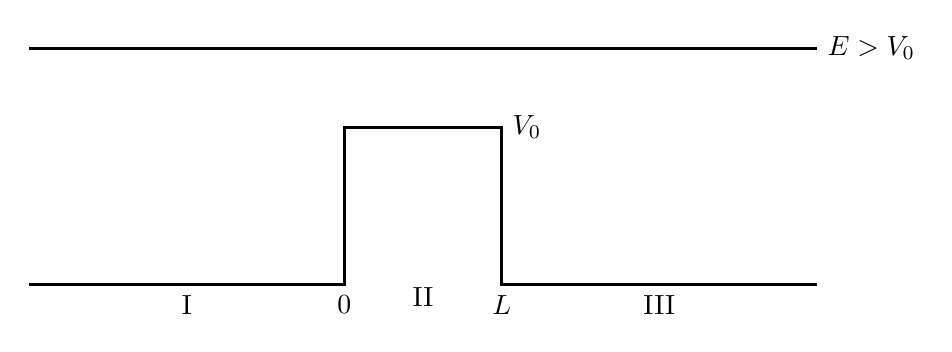
\begin{tikzpicture}
            \draw[very thick] (-4,-2) -- (0,-2) node[midway,below] {I} node[anchor=north] {$0$} -- (0,0) -- (2,0) node[midway,below,yshift=-1.9cm] {II} node[anchor=west] {$V_0$} -- (2,-2) node[anchor=north] {$L$} -- (6,-2) node[midway,below] {III} (-4,1) -- (6,1) node[anchor=west] {$E > V_0$};
        \end{tikzpicture}
    \end{center}

    \begin{enumerate}[(a)]
        \item Show that the analysis of the scattering by a one-dimensional \textit{well} in section 9-4 leads to equations identical in form to those of the present case, so that the general result (Eq. 9-12) applies to the barrier also. 
        
        \begin{solution}
            Here, we have three regions, and so we have

            \begin{align*}
                \psi_1(x) &= A_0 e^{ik_1x} + Ae^{ik_2x}\\
                \psi_2(x) &= Be^{ik_2x} + Ce^{-ik_2x}\\
                \psi_3(x) &= De^{ik_1x}
            \end{align*}

            And for continuity, we derive the set of equations at $x = 0$: 

            \begin{align*}
                A_0 + A &= B + C\\
                ik_1(A_0 - A) &= ik_2(B - C)
            \end{align*}

            And at $x = L$: 

            \begin{align*}
                Be^{ik_2L} + Ce^{-ik_2L} &= De^{ik_2}\\
                k_2(Be^{ik_2L} - Ce^{ik_2L}) &= ik_1De^{ik_1L}
            \end{align*}

            These are the same set of equations that we had to solve for the scattering case of the finite square well, and so therefore the general result also applies to the barrier.
        \end{solution}
        \item For the special cases $E \gg V_0$ and $k_2L = n\pi$ treated in Section 9-4, show that the results are the same as for the present case. The case $k_1 \ll k_2$ for the well cannot apply to the barrier. Instead consider the case $k_2 \to 0$ and show that the resulting transmission coefficient is the same as that calculated in the next exercise (``Skimming a barrier'')
        
        \begin{solution}
            For the case where $E \gg V_0$, then we get $k_1 \approx k_2$, so we get the transmission to be: 

            \[ T = \left|\frac{4k_1^2}{4k_1^2e^{-ik_1L}}\right|^2 = 1\] 

            This makes sense, because when the energy is significantly larger than the barrier, we can think of this as nearing the situation where the barrier is nonexistent, where we expect the transmission to be 1. 

            For the case where $k_2L = n\pi$, then we get the fact that $e^{ik_2L} = e^{-k_2L} = \pm 1$, depending on whether $n$ is even or odd. What matters here is that their magnitude is 1, meaning that our equation simplifies to: 

            \[ T = \left| \frac{4k_1k_2}{(k_1 + k_2)^2 - (k_2 - k_1)^2}\right|^2 = \left| \frac{4k_1k_2}{4k_1k_2}\right|^2 = 1\] 

            Again, this makes sense because the width of the barrier is an integer multiple of $\lambda$, giving us destructive interference over the barrier, and so reflection goes to 0. 

            For the case where $k_2 \to 0$, then this is referring to the case where $E \approx V_0$, and so $\epsilon \approx 1$. Therefore, our tranmission probability becomes: 

            \[ T \approx  \frac{4(2)}{4(2) + \sin^2(\beta \sqrt{2})} = \frac{8}{8 + \sin^2\left( \frac{L\sqrt{2mV_0} \sqrt{2}}{\hbar}\right)}\] 

            If we take the approximation that $\sin^2 \theta \approx \theta^2$, then we can get the equation: 

            \[ T \approx \frac{8}{8 + \frac{4L^2mV_0}{\hbar^2}}\] 

            which is the same expresion that we get in problem 5(b). 
        \end{solution}
    \end{enumerate}

    \pagebreak

    \section*{Problem 5}

    Find the fraction of incident particles transmitted by a rectangular potential barrier in the very special case that the energy $E$ of the incident particles is exactly equal to the barrier height $V_0$. Let $k$ stand for the wave number of the incident particles and $L$ stand for the barrier width. 

    \begin{center}
        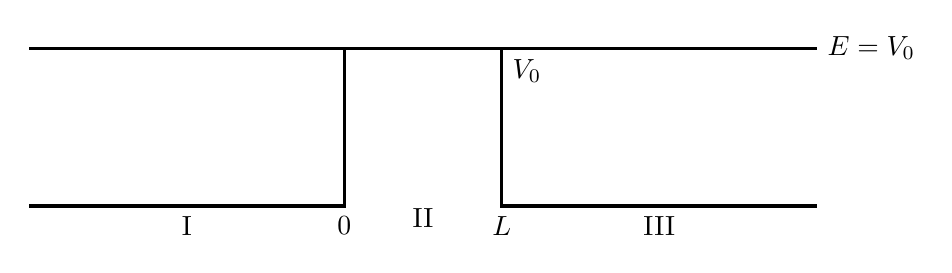
\begin{tikzpicture}
            \draw[very thick] (-4,-2) -- (0,-2) node[midway,below] {I} node[anchor=north] {$0$} -- (0,0) -- (2,0) node[midway,below,yshift=-1.9cm] {II} node[anchor=north west] {$V_0$} -- (2,-2) node[anchor=north] {$L$} -- (6,-2) node[midway,below] {III} (-4,0) -- (6,0) node[anchor=west] {$E = V_0$};
        \end{tikzpicture}
    \end{center}

    \begin{enumerate}[(a)]
        \item Starting from the \schrodinger equation, show directly that the form of the wave function inside the barrier is linear: 
        \[ \psi_2(x) = Bx + C\]

        (In general, $B$ and $C$ may be complex numbers, so it is not strictly correct to say that $\psi_2$ represents a ``straight line'' in the usual sense.)


        \begin{solution}
            The \schrodinger equation reads: 

            \[ \left[ \frac{\hbar^2}{2m} + V_0\right] \psi = E\psi\]

            And since $E = V_0$, then we get: 

            \[ \frac{\partial^2}{\partial x^2} \psi(x) = 0\] 

            The most general form of $\psi$ is therefore $\psi(x) = Bx + C$ for this situation, as desired. 
        \end{solution}

        \item Set up and solve the bounary doncition equations to obtain an expression for the transmission coefficient. Does this expression have the expected limiting values for $L = 0$ and $L \to \infty$?
        
        \begin{solution}
            Matching coefficients at $x = 0$ and $x = L$: 

            \begin{align*}
                A_0 + A &= C\\
                ik_1(A_0 - A) &= B\\
                BL + C &= De^{ik_1L}\\
                B &= ik_1De^{ik_1L}
            \end{align*}

            Combining the first two equations, we get 

            \begin{equation} \label{eq1}
                2A_0 = C + \frac{B}{ik_1}
            \end{equation}

            and combining the last two equations we get: 

            \begin{equation} \label{eq2}
                C = (1 - ik_1L)De^{ik_1L}
            \end{equation}

            And so therefore, we get: 

            \begin{align*}
                T = \left|\frac{D}{A_0}\right|^2 &= \left|\frac{2}{(2 - ikL)e^{ik_1L}}\right|^2\\
                &= \frac{4}{4 + k_1^2L^2}\\
                &= \frac{4}{4 + \frac{2mV_0L^2}{\hbar^2}}
            \end{align*} 

            Here, we can now analyze the edge cases. For $L = 0$, we get $T = 1$, which makes sense, since no barrier means that the transmission is guaranteed. On the flip side, as $L \to \infty$, we get $T = 0$, which also makes sense, since an infinitely long barrier means no transmission is possible. 
        \end{solution}
        \item For thwa what value of $L/\lambda$ (where $\lambda$ is the de Broglie wavelength) is the transmission equal to $\frac 12$?
        

        \begin{solution}
            We have the relation that $\lambda = \frac{2\pi\hbar}{\sqrt{2mE}}$, and so the transmission becomes: 

            \[ T = \frac{4}{4 + \frac{2mV_0L}{\hbar^2}} = \frac{1}{2}\] 

            Solving this equation gives the result that 

            \[ \frac{L}{\lambda} = \frac{1}{\pi}\] 
        \end{solution}
    \end{enumerate}
\end{document}